% Basic stuff
\documentclass[a4paper,11pt]{article}
\usepackage{scrextend}

% 3 column landscape layout with fewer margins
\usepackage[landscape, left=0.75cm, top=0.75cm, right=0.75cm, bottom=1cm, footskip=15pt]{geometry}
\usepackage{flowfram}
\usepackage{bbm}
\ffvadjustfalse
\setlength{\columnsep}{0.5cm}
\Ncolumn[<10]{4}
\onecolumn[10]

% define nice looking boxes
\usepackage[many]{tcolorbox}
\changefontsizes[11pt]{11pt}

% a base set, that is then customised
\tcbset {
	base/.style={
		boxrule=0mm,
		leftrule=1mm,
		left=1.75mm,
		arc=0mm, 
		fonttitle=\bfseries, 
		colbacktitle=black!10!white, 
		coltitle=black, 
		toptitle=0.75mm, 
		bottomtitle=0.25mm,
		title={#1}
	}
}

\definecolor{brandblue}{rgb}{0.34, 0.7, 1}
\newtcolorbox{mainbox}[1]{
	colframe=brandblue, 
	base={#1}
}

\newtcolorbox{subbox}[1]{
	colframe=black!20!white,
	base={#1}
}

% Mathematical typesetting & symbols
\usepackage{amsthm, mathtools, amssymb} 
\usepackage{marvosym, wasysym}
\allowdisplaybreaks

% Tables
\usepackage{tabularx, multirow}
\usepackage{makecell}
\usepackage{booktabs}
\renewcommand*{\arraystretch}{2}

% Make enumerations more compact
\usepackage{enumitem}

% To include sketches & PDFs
\usepackage{graphicx}

% For hyperlinks
\usepackage{hyperref}
\hypersetup{
	colorlinks=true
}
\renewcommand{\baselinestretch}{.9}
% Metadata
\title{Cheatsheet\\ Introduction to Machine Learning}
\author{Thomas Gassmann}
\date{\vspace{-10pt}Sommer 2024}

% Math helper stuff
\def\limxo{\lim_{x\to 0}}
\def\limxi{\lim_{x\to\infty}}
\def\limxn{\lim_{x\to-\infty}}
\def\R{\mathbb{R}}
\def\P{\mathbb{P}}
\def\F{\mathcal{F}}
\def\sumn{\sum_{n=0}^\infty}
\def\sumk{\sum_{k=1}^\infty}
\def\E{\mathbb{E}}
\DeclareMathOperator{\Var}{\text{Var}}
\newcommand{\middot}{~\textperiodcentered~}
\newlist{rowlist}{enumerate*}{1}
\setlist[rowlist]{label={\textbf{\roman*}\text{: }}, afterlabel={}, itemjoin=\middot}

\newcommand{\C}{\mathbb{C}}
\newcommand{\K}{\mathbb{K}}
\newcommand{\N}{\mathbb{N}}
\newcommand{\Q}{\mathbb{Q}}
\newcommand{\Z}{\mathbb{Z}}
\newcommand{\X}{\mathbb{X}}
\renewcommand{\P}{\mathbb{P}}

\newcommand{\No}{\mathcal{N}}

\newcommand{\br}{\par\medskip\noindent}
% \newcommand{\P}{\mathbb{P}}
\newcommand{\Oh}{\mathcal{O}}
% \newcommand{\vphi}{\varphi}
% \newcommand{\veps}{\varepsilon} 
\newcommand{\bd}{\textbf}
\newcommand{\equi}{\Leftrightarrow}
\newcommand{\imp}{\Rightarrow}
\newcommand{\emp}{\varnothing}
\newcommand{\subs}{\subseteq}
\newcommand{\ol}{\overline}
\newcommand{\ra}{\rangle}
\newcommand{\la}{\langle}
\newcommand{\ox}{\otimes}
\newcommand*\dx{\mathop{}\!\mathrm{d}x}
\newcommand*\dy{\mathop{}\!\mathrm{d}y}
\newcommand*\dz{\mathop{}\!\mathrm{d}z}

\DeclareMathOperator*{\argmax}{arg\,max}
\DeclareMathOperator*{\argmin}{arg\,min}
\DeclareMathOperator*{\vol}{vol}
\DeclareMathOperator*{\Mat}{Mat}

\setlength{\parindent}{0pt}

\makeatletter
\renewcommand{\section}{\@startsection{section}{1}{0mm}%
                                {0pt}%
                                {0.5pt}%x
                                {\sffamily\bfseries\large}}
\renewcommand{\subsection}{\@startsection{subsection}{1}{0mm}%
                                {0pt}%
                                {0.1pt}%x
                                {\sffamily\bfseries}}
\begin{document}
\small


\begin{center}
    Lizenziert unter CC BY-SA 4.0. Für Urheber, Quellen und Lizenzinformationen, siehe:\\
    \href{https://github.com/thomasgassmann/eth-cheatsheets}{github.com/thomasgassmann/eth-cheatsheets}

    GITCOMMIT
\end{center}


\section*{General}

$$
\operatorname{var}(AX)=A\operatorname{var}(X)A^\top
$$

$$
\begin{bsmallmatrix}
a&b \\ 
c&d
\end{bsmallmatrix}^{-1}=\frac{1}{ad-bc}
\begin{bsmallmatrix}
d&-b \\ 
-c&a
\end{bsmallmatrix}
$$

$$
\widehat{\operatorname{cov}}(X)=\frac{1}{n}X^\top X=\frac{1}{n}\sum_i x_ix_i^\top
$$

\subsection*{Convexity}
\begin{itemize}
    \item{$f(t x + (1-t)y) \leq t f(x) + (1-t) f(y)$}
    \item{$f$ convex, $g$ affine $\imp f\circ g$ convex}
    \item{$f$ convex, non-decreasing, $g$ convex $\imp f\circ g$ convex}
    \item{$f$ convex, $g$ affine $\imp f\circ g$ convex}
    \item{$\alpha, \beta \geq 0, f, g$ convex $\implies \alpha f + \beta g$ convex}
    \item pointwise maximum of two convex functions is convex
\end{itemize}

\subsection*{Gaussian}

For $\mu \in \R^p, \Sigma \in \R^{p \times p} \ \text{spd}$, $X$ has normal distribution with density:

$\frac{1}{\sqrt{(2\pi)^p \det(\Sigma))}}\exp({-\frac{1}{2}(x-\mu)^\top \Sigma^{-1}(x-\mu)})$

\subsection*{PSD}
$M \in \mathbb{R}^{n\times n}$ PSD $\Leftrightarrow \forall x \in \mathbb{R}^n: x^\top Mx \geq 0 \\
\Leftrightarrow$ all principal minors of $M$ have non-negative determinant\\
$\Leftrightarrow \lambda \geq 0 \ \forall \lambda\in\sigma(M)$

\subsection*{Expected estimation and generalization error}
$\E_{X}\ell(f(X), f^\ast(X))$ \\ 
$\E_{X,Y}\ell(f(X), Y)$

\subsection*{Central Limit Theorem}

Für $X_i$ iid mit $m = \E[X_1]$ und $\Var[X_1] = \sigma^2$ gilt $\P\left[\frac{\sum_{i=1}^n X_i - n m}{\sqrt{\sigma^2 n}} \leq a\right] \xrightarrow[n \to \infty]{} \Phi(a)$.

\subsection*{Gradient Descent}
$w_{t+1} = w_t - \eta \nabla L(w_t)$
\subsection*{Gradient Descent with Momentum} $w_{t+1}=w_t+m(w_t-w_{t-1})-\eta \nabla L(w_t)$
\subsection*{SGD}
Pick data poi nt $(x,y)$ u.a.r. and set\\  $w_{t+1} = w_t - \eta \nabla L_{(x,y)}(w_t)$ \\ For mini-batch SGD, choose $S \subseteq \{1, \ldots, n\}$ and set $w_{t+1} = w_t - \eta \nabla L_{S}(w_t)$
\subsection*{Complexity}
Matmul $A\in\R^{n\times k},B\in R^{k\times d}$: $\Theta(n k d)$

\subsection*{KL Divergence}
$D_{KL}(P||Q) = \mathbb{E}_p[\log(\frac{p(x)}{q(x)})]$, 0 iff $P = Q$, always non-negative
\\

\section*{Regression}
\subsection*{Linear Regression}
$w^* = \operatorname{argmin_w} \|y - Xw\|^2=(X^T X)^{-1} X^T y\\
\nabla_w \hat{R}(w) = -2 \sum_{i=1}^n (y_i-w^T x_i) \cdot x_i\\
= 2X^T (Xw-y)$


\subsection*{Ridge}
$w^*=\argmin_w \|y - Xw\|^2 + \lambda ||w||_2^2\\
w^*=(X^T X + \lambda I)^{-1} X^T y\\
\nabla_w \hat{R}(w) = 2X^T (Xw-y) + 2\lambda w$

\subsection*{LASSO}
$w^*=\argmin_w \|y - Xw\|^2 + \lambda ||w||_1$
\\
\section*{Classification}
\subsection*{Logistic Loss}
$\ell_{log}(x,y) = \log(1+e^{-yf(x)})$ (convex)\\
$\nabla_w \ell_{log}(x,y) = \frac{-y\nabla_w f(x)}{1+\exp(yf(x))} $

\subsection*{Hinge Loss}
$l_H(x,y,w) = \max \{0,1-y w^\top x\}$ (convex)\\
$\nabla_w l_H = \begin{cases}
    -y x&\text{ , if $yw^\top x<1$}\\
	0 &\text{ , if $y w^\top x \geq 1$}
\end{cases}$

\subsection*{Hard-margin SVM}
If data is separable, find \\
$\min_w \lVert w \rVert_2 \ \text{s.t.} \ y_iw^\top x_i\geq 1 \ \forall i.$\\

\subsection*{Soft-margin SVM}
If data is not separable, find \\
$\min_{w,\xi}\frac{1}{2}\|w\|^2  +\lambda\sum_i\xi_i\ \ \ 
\text{s.t.} \begin{cases}
    y_iw^\top x_i\geq 1-\xi_i\\
    \xi_i\geq0
\end{cases}\\
=\min_w\frac{1}{2}\|w\|^2+\lambda\sum_i\max \{0,1-y_i w^\top x_i\}$


\subsection*{Evaluation}
Accuracy $=\frac{TP+TN}{TP+TN+FP+FN}$\\
Precision $=\frac{TP}{TP+FP} = 1-$ FDR = $\frac{TP}{|\{\hat{y} = +1\}|}$\\
FDR = $\frac{FP}{|\{\hat{y} = +1\}|}$, Recall $=$ TPR$ =\frac{TP}{TP+FN}$\\
FPR $=\frac{FP}{TN+FP} = \frac{FP}{|\{y = -1\}|}$\\
FNR $=\frac{FN}{|\{ y = +1 \}|}$\\
TPR $=\frac{TP}{|\{ y = +1 \}|}$, TNR $=\frac{TN}{|\{ y = -1 \}|}$\\
ROC curve: \ \ $x=$ FPR, $y=$ TPR\\
F1 $=\frac{2TP}{2TP+FP+FN}=\frac{2}{1/Precision+1/Recall}$\\
\hspace*{-5mm}
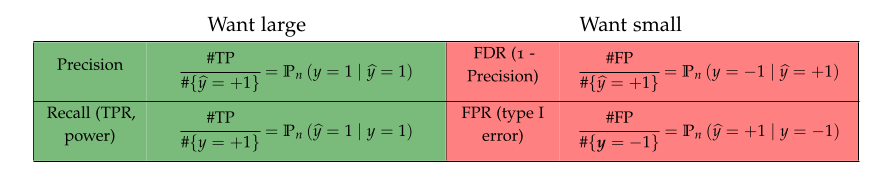
\includegraphics[width=1.1 \linewidth]{matrix.png}

\section*{Kernels}
\subsection*{Polynomial kernel}
$k(x,y) = (x^Ty)^m$  all monomials of deg. m \\
$k(x,y) = (1+x^Ty)^m$ all monomials up to deg. m
There are $\binom{d+m}{m}=O_d(d^m)=O_m(m^d)$ monomials of 
order $m$ in $d$ variables.

\subsection*{Properties $k(x,y) = \phi(x)^T\phi(y)$}
\begin{enumerate}[noitemsep,leftmargin=*,topsep=0pt,parsep=0pt,partopsep=0pt]
    \item $k$ must be symmetric.
    \item Kernel matrix $K$ must be PSD for all $x_1,\dots,x_n$.\\
$K=\begin{bmatrix}
    k(x_1,x_1)&\dots&k(x_1,x_n) \\ 
    \vdots&\ddots&\vdots\\
    k(x_n,x_1)&\dots&k(x_n,x_n)
    \end{bmatrix}
$\end{enumerate}

\subsection*{Valid kernels}
$k_1 + k_2,$
$k_1 k_2,$
$  c k$ if $c>0;$\\
$f(k)$, where $f$ is a polynomial/power series with non-negative coefficients;\\
$k(\binom{x}{y}, \binom{x'}{y'})=k(x,x')k(y,y'),\\ 
k(\binom{x}{y}, \binom{x'}{y'})=k(x,x') + k(y,y')$ \\
where $\binom{x}{y}$ is concatenation of vectors;\\
$k(x,y)=g(x)k(x,y)g(y)$ where $g\colon X\to\R$.


\subsection*{Kernelized Ridge}
Ansatz: $w^*=\Phi^\top\alpha$\\
$\min_w\|\Phi w-y\|^2 + \lambda ||w||_2^2\\
=\min_a ||K\alpha -y||_2^2 + \lambda \alpha^T K \alpha$\\
$\alpha^*=(K+\lambda I)^{-1} y$\\
Prediction: $\hat{y} = \Sigma_{i=1}^n \alpha_i^* k(x_i,x)$\\
\section*{Neural Networks}
$F(x)=W^{L}\phi^{L-1}(W^{L-1}...(\phi^{1}(W^{1}x)...))$

\subsection*{Activation functions}
Sigmoid: $\varphi(z) = \frac{1}{1+\exp(-z)}$;  $\varphi' = (1 - \varphi)\cdot\varphi$\\
Tanh: $\tanh(z) = \frac{\exp(z)-\exp(-z)}{\exp(z)+\exp(-z)}$\\
ReLu:  $\max(0,z)$

\subsection*{Backpropagation}
For the output layer $L$:
\begin{enumerate}[noitemsep,leftmargin=6mm,topsep=0pt,parsep=0pt,partopsep=0pt]
\item Compute error $\delta^{L} = \nabla_f\ell$
\item and gradient $\nabla_{W^L}\ell=\delta^L(v^{(L-1)})^\top$
\end{enumerate}
For each hidden layer $l=L-1,...,1$:
\begin{enumerate}[noitemsep,leftmargin=6mm,topsep=0pt,parsep=0pt,partopsep=0pt]
\item  Compute error $\delta^{l} =\varphi'(z^l)\odot ((W^l)^\top \delta^{l+1})$
\item and gradient $\nabla_{W^l}\ell=\delta^l(v^{(l-1)})^\top$
\end{enumerate}

\subsection*{Regularization}
\begin{itemize}[noitemsep,leftmargin=6mm,topsep=2pt,parsep=2pt,partopsep=2pt]
    \item Weight decay
    \item Early stopping (validation)
    \item Dropout
    \item Batch normalization
\end{itemize}

\subsection*{CNNs}
Output size (per dim) $l=\frac{n+2p-f}{s}+1$
\\
\section*{Clustering}
\subsection*{k-means}
Want $\mu_i$ to minimize $\sum_{i=1}^n \min_{j\in\{1,...k\}}\|x_i-\mu_j\|_2^2$
Non-convex and NP-hard in general. Can be kernelized.

\subsection*{Lloyd's heuristic}
While not converged:\\
$\hspace*{3mm}z_i = \argmin_{j\in\{1,...,k\}}\|x_i - \mu_j^{t-1}\|_2^2\\
\hspace*{3mm}\mu_j^{(t)} = \frac{1}{n_j}\sum_{i:z_i=j}x_i$\\
Monotonically decreases objective and converges to a local 
optimum. Cost per iteration $O(nkd)$.

\section*{Dimension Reduction}
\subsection*{Principal component analysis (PCA)}
Given centered data, the PCA problem is 
$$\min_{W^TW=I_k,z_i\in\R^k}\sum_{i=1}^n||W z_i - x_i||_2^2,$$
with solution $W^* = (v_1|...|v_k)$ where $v_i$ are the ordered 
eigenvectors of $\frac{1}{n}\sum_ix_ix_i^T$ 
and $z_i = {W^*}^\top x_i$. 

\subsection*{Kernel PCA}
The Kernel Principal Components are given by $\alpha^{1},...,\alpha^{k}\in \mathbb{R}^n$ 
where $\alpha^{i} = \frac{1}{\sqrt{\lambda_i}}v_i$ and 
$K = \sum_{i=1}^n \lambda_i v_i v_i^T$ with ordered $\lambda_i.$ A point 
$x$ is projected to $z \in \mathbb{R}^k$:
$z_i = \sum_{j=1}^n\alpha_j^{(i)}k(x,x_j)$

\subsection*{Autoencoders}
Try to learn identity function $x \approx f(x;\theta)
= f_2(f_1(x_1;\theta_1);\theta_2)$. NN Autoencoder with 
linear activations is equivalent to PCA.
\\
\section*{Probabilistic Modeling}
\subsection*{MLE}
Given a choice of marginal $P(Y|X,\theta)$ take 
$\theta^* =\argmax_\theta \prod_{i=1}^n {P_\theta}(y_i|x_i).$

\subsection*{Bayes optimality}
$\argmin_f\E_{x,y}[(y-f(x))^2]=\E[Y\mid X]$\\
$\argmin_f\E_{x,y}[1_{[y\neq f(x)]}]\\=\argmax_yp(Y=y\mid X=x)$

\subsection*{Bias-Variance-noise decomposition}
$\E_{x,y}[(\hat{f}_D(x)- y)^2]\\=
\E_x[\E_D[\hat{f}_D(x)]-f^*(x)]^2\\
\hspace*{0.1mm}+\E_x[\operatorname{var}[\hat{f}_D(x)]]\\
\hspace*{0.1mm}+\E_{x,y}[(y-f^*(x))^2]$ where $f^*=\E[Y\mid X]$.


\subsection*{Logistic regression}
Parametrize $P(y\mid x)$ by $\frac{1}{1+\exp(-y w^\top x)}$.\\
MLE is $\operatorname{argmax_w} P(y_{1:n}|w,x_{1:n})\\
= \operatorname{argmin_w} - \sum_{i=1}^n \log P(y_i|w,x_i)\\
= \operatorname{argmin_w} \sum_{i=1}^n \log(1+\exp(-y_i w^\top x_i))$

\subsection*{Gradient for logistic regression}
$\ell(w) = \log(1+\exp(-yw^\top x))$\\
$\nabla_w \ell(w) =\frac{-yx}{1+\exp(yw^\top x)}$

\subsection*{Multiclass Logistic Regression}
Parametrize $P(Y=i\mid x)$ by $\frac{\exp(w_i^\top x)}{\sum_j \exp(w_j^\top x)}$.

\subsection*{Kernelized logistic regression}
$\min_\alpha\sum_i\log(1+\exp(-y_i\alpha^\top K_i)) + \lambda\alpha^\top K \alpha$
$\hat{P}(y\mid x)=\frac{1}{1+\exp(-y\sum_i\alpha_ik(x_i,x))}$
\\
\section*{Bayesian decision theory}
\begin{enumerate}[noitemsep,leftmargin=6mm,topsep=0pt,parsep=0pt,partopsep=0pt]
	\item Conditional distribution over labels $P(y|x)$
	\item Set of actions $\mathcal{A}$
	\item Cost function $C:Y\times \mathcal{A} \rightarrow \mathbb{R}$
\end{enumerate}

Pick action that minimizes the expected cost:
$a^* = \operatorname{argmin_{a \in \mathcal{A}}} \mathbb{E}_y[C(y,a)|x]$

\subsection*{Optimal decision for logistic regression}
$a^* = \operatorname{argmin_y} \hat{P}(y|x) = sign(w^\top x)$ assuming 
$0$-$1$-cost.
\\
\section*{Generative Modeling}
Discriminative: Estimate $P(y\mid x)$\\
Generative: Estimate $P(y,x)$

Typical approach to generative modeling:
\begin{enumerate}[noitemsep,leftmargin=6mm,topsep=2pt,parsep=2pt,partopsep=2pt]
    \item Estimate prior on labels $P(y)$
    \item Estimate conditional distribution $P(x\mid y)$ for each class y
    \item Obtain predictive distribution using Bayes' rule:
$P(y\mid x) = \frac{P(y) P(x\mid y)}{P(x)} = \frac{P(x,y)}{P(x)}$
\end{enumerate}

\subsection*{Naive Bayes}
Naive Bayes assumes conditional independence:
$$P(X_1,...,X_n\mid Y) = \prod_i P(X_i\mid Y).$$
If independence is violated, predictions become overconfident (close to 0 and 1).

\subsection*{Decision rule}
$\hat{y} = \operatorname{argmax_{y}} P(y\mid x)\\
\hspace*{2.1mm}= \operatorname{argmax_{y}} P(y) \prod_{i} P(x_i\mid y)\\
\hspace*{2.1mm}= \operatorname{argmax_{y}} \log P(y) + \sum_{i} \log P(x_i\mid y)$

\subsection*{QDA/Gaussian Bayes Classifier}
$P(Y=y) = p_y$ and $P(x\mid y) = \mathcal{N}({\mu}_y, {\Sigma}_y)$\\
$\hat{p}_y= \frac{\operatorname{Count(Y = y)}}{n}$\\
$\hat{\mu}_{y} = \frac{1}{\operatorname{Count}(Y=y)} \sum_{i:y_i=y} {x_i} $\\
$\hat{\Sigma}_{y} = \frac{1}{\operatorname{Count}(Y=y)} \sum_{i:y_i=y} (x_i - \hat{\mu}_{y})(x_i-\hat{\mu}_y)^T $

For two classes $\hat{y} = \operatorname{sign}\Big(\log\frac{P(Y=1\mid x)}{P(Y=-1\mid x)}\Big) $ 
\\ where  
$    \log\frac{P(Y=1\mid x)}{P(Y=-1\mid x)} = \log \frac{\hat{p}}{1-\hat{p}} + \frac{1}{2}\log \frac{|\hat{\Sigma}_-|}{|\hat{\Sigma}_+|}\\
    + \frac{1}{2}(x - \hat{\mu}_-)^T \hat{\Sigma}_-^{-1} (x - \hat{\mu}_-) - \frac{1}{2}(x - \hat{\mu}_+)^T \hat{\Sigma}_+^{-1} (x - \hat{\mu}_+)$

\subsection*{Gaussian Naive Bayes}
GBC with diagonal $\Sigma$s. GNB with shared $\Sigma$s across
two classes yields the same predictions as Logistic Regression
(if model is true).

\subsection*{Fisher's LDA (Subcase of GBC)}
Assume: Two classes, $p = 0.5$, ${\Sigma}_- = {\Sigma}_+ $

\subsection*{Outlier Detection}
Classify $x$ as outlier if $P(x) \leq \tau$.

\subsection*{Regularization}
\begin{itemize}[noitemsep,leftmargin=6mm,topsep=0pt,parsep=0pt,partopsep=0pt]
    \item Restricting model (i.e. covariance)
    \item Prior on parameters.\\
\end{itemize}

\section*{Mixture Models}
\subsection*{Gaussian Mixtures}
$P(x\mid z) = \sum_iw_i\mathcal{N}({\mu}_i, {\Sigma}_i)$\\
MLE is a nonconvex problem $\rightarrow$ EM.

\subsection*{Hard-EM}
\textbf{E-step: } Compute \\$z_i^{(t)} = \operatorname{argmax_z} P(z\mid x_i, \theta^{(t-1)})\\
\hspace*{1.4mm}= \operatorname{argmax_z} P(z\mid \theta^{(t-1)}) P(x_i\mid z,\theta^{(t-1)})\\
 \stackrel{\text{GMM}}{=}\operatorname{argmax_z} w_z^{(t-1)}\mathcal{N}(x;\ \mu_z^{(t-1)},\Sigma_z^{(t-1)})$\\
\textbf{M-step: }
$\theta^{(t)} = \operatorname{argmax_\theta} P(x_{1:n},z^{(t)}_{1:n}\mid \theta)$\\
Hard-EM converges to a local maximum
of $P(x_{1:n},z^{(t)}_{1:n}\mid \theta)$. It tends to do poorly if clusters overlap. 
Hard-EM for GMM with $w_z=\frac{1}{k}, \Sigma_z=\sigma^2{I}$
is equivalent to k-means.

\subsection*{Soft-EM}
\textbf{E-step: \newline} Compute the distribution of $Z\mid x,\theta^{(t-1)}$, i.e. for each $x$ the responsibilities
\begin{equation*}
    \begin{aligned}
        P_{\theta^{(t-1)}}(Z=j\mid x) &= \frac{P(Z=j)P(x\mid Z=j)}{P(x)} \\
        &\stackrel{\text{GMM}}{=}
        \frac{w_j \mathcal{N}(x;\ \Sigma_j,\mu_j)}{\sum_k w_k \mathcal{N}(x;\ \Sigma_k,\mu_k)}.
    \end{aligned}
\end{equation*}

\textbf{M-step:} 
\begin{equation*}
    \begin{aligned}
        \theta^{(t)}&=\argmax_\theta 
        \mathbb{E}_{Z_{1:n}\mid x_{1:n},\theta^{(t-1)}}
        \big[\log P_\theta(x_{1:n},Z_{1:n})\big]\\
        &\stackrel{\text{iid\&cond.ind.}}{=}
        \sum_{i=1}^n \mathbb{E}_{Z_i\mid x_i,\theta^{(t-1)}}
        \big[\log P_\theta(x_i,Z_i)\big] \\
        &= \sum_{i=1}^n \sum_{j=1}^k P_{\theta^{(t-1)}}(Z_i=j\mid x_i)\log P_\theta(x_i,Z_i=j)
    \end{aligned}
\end{equation*}

GMM M-step:\\ $w_j^{(t)} \leftarrow \frac{1}{n} \sum_{i} \gamma_j^{(t)} (x_i)$; \\
$\mu_j^{(t)} \leftarrow \frac{\sum_{i} \gamma_j^{(t)} (x_i) x_i}{\sum_{i} \gamma_j^{(t)} (x_i)}\\
\Sigma_j^{(t)} \leftarrow \frac{\sum_{i} \gamma_j^{(t)}(x_i) (x_i - \mu_j^{(t)}) (x_i - \mu_j^{(t)})^\top}{\sum_{i} \gamma_j^{(t)}(x_i)} \{+\nu^2\mathbb{I}\}$\\ %\text{|}\gamma^{(t) = \gamma}$

The cluster size can be selected via CV.
EM converges to a local maximum for GMMs, dependent on
initialization.
\subsection*{Semi-Supervised Learning w/ GMMs:}
Set $P_{\theta^{(t-1)}}(Z=j\mid x) =1_{\{j = y\}}$ for labeled points
$(x,y).$
\\

\section*{GANs}
Goal: Approximate a distribution $X\approx G_w(Z)$ where $Z$
is a simple distribution.
Train $G$ and $D$ simultaneously 
on the objective
$$\min_G\max_D\E_x[\log D(x)] +\E_Z[\log1-D(G(Z))].$$
Training requires finding a saddle point. If 
$G, D$ are complex enough, then the distribution of $X$
minimizes the objective. Cannot compute likelihood on holdout set.
If $D$ is globally optimal for some $G$, then $D$ predicts
$\frac{p_X(x)}{p_G(x)+p_X(x)}$.

\end{document}
